\section{Introduction}
Understanding the in-vivo kinematics of total joint replacement has been essential in implant design, post-operative assessment, and predicting wear and failure patterns for nearly three decades \cite{freglyComputationalWearPrediction2005,banks2003HapPaul2004,banksRationaleResultsFixedBearing2019}.
Recent advancements in computer vision and machine learning have enabled these analyses for total knee arthroplasty (TKA) in a fully autonomous and clinically practical setting, utilizing single-plane fluoroscopy \cite{brobergValidationMachineLearning2023,jensenJointTrackMachine2023}.
However, using only a single camera inherently limits the measurement accuracy due to loss of depth perception and the introduction of ambiguous projected shapes during optimization \cite{floodAutomatedRegistration3D2018,mahfouzRobustMethodRegistration2003,zuffiModelbasedMethodReconstruction1999,banksAccurateMeasurementThreedimensional1996}.
The observed limitation, predominantly impacting mediolaterally symmetric tibial implants, led to a phenomenon termed “symmetry traps.”
In such instances, two distinct three-dimensional orientations of the implant produce indistinguishable two-dimensional projected geometries.
A machine learning algorithm was developed to address these symmetry traps in symmetric tibial implants.
This algorithm was trained to recognize accurate anatomic orientations and correct images caught in optimization minima \cite{jensenCorrectingSymmetricImplantInReview}.
However, this approach required the symmetric implant to register into one of the two potential local minima, each corresponding to a distinct “symmetry trap.”

The application of the same optimization routine and cost function \cite{floodAutomatedRegistration3D2018,jensenJointTrackMachine2023} to reverse total shoulder arthroplasty (rTSA) resulted in significantly lower performance compared to its application in TKA implants \cite{jensenJointTrackMachine2023}.
This suboptimal performance manifested primarily along the internal/external rotation axis, which has salient features often occluded by the glenosphere implant in frontal-plane fluoroscopy (\cref{fig:bad_ie_hum}).
Additionally, this axis is nearly rotationally symmetric for both the humeral and glenospere implants.
Poor rotation registration also increases translation errors, as the silhouette shape of the estimated pose is wholly different from the fluoroscopic image, causing imprecise translation alignment along all axes.
In a manual registration setting \cite{muJointTrackOpenSourceEasily2007}, different combinations of model and image views are utilized to overcome these limitations (\cref{fig:TSA-multiview}).

\begin{table}
	\caption{Root mean squared differences between JointTrack Machine Learning optimized kinematics and manually registered kinematics on single-plane fluoroscopy} \label{tab:jtml-tsa-tka-vals}
	\begin{tabularx}{\linewidth}{|X|X|X|X|X|X|X|}\hline
		{\bf Implant Type} & $x_{trans} (mm)$ & $y_{trans} (mm)$ & $z_{trans} (mm)$ & $x_{rot} (^{\circ})$ & $y_{rot} (^{\circ})$ & $z_{rot} (^{\circ})$ \\ \hline
		Humeral            & 8.46             & 8.64             & 152.78           & 22.59                & 64.74                & 11.81                \\\hline
		Glenosphere        & 0.97             & 1.44             & 32.58            & 13.72                & 26.40                & 8.30                 \\\hline
		Femoral            & 0.57             & 0.39             & 26.95            & 0.66                 & 0.73                 & 0.60                 \\\hline
		Tibial             & 0.67             & 0.64             & 27.17            & 1.63                 & 2.74                 & 0.66                 \\\hline
	\end{tabularx}
\end{table}


\begin{figure}[h!]
	\centering
	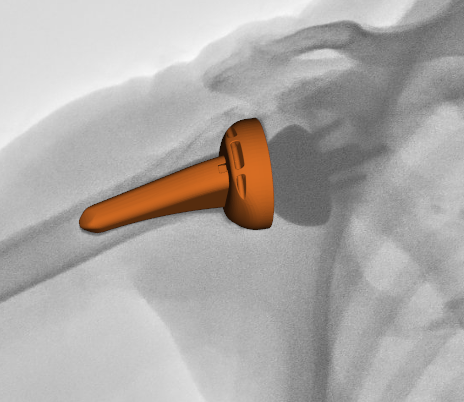
\includegraphics[width=0.4\textwidth]{~/figures/raster/BAD_IE_HUM.png}
	\caption{A representative example of poor internal/external rotation of the humeral implant after automated model-image registration using JointTrack Machine Learning \cite{jensenJointTrackMachine2023}.}
	\label{fig:bad_ie_hum}
\end{figure}


\begin{figure}[h!]
	\centering
	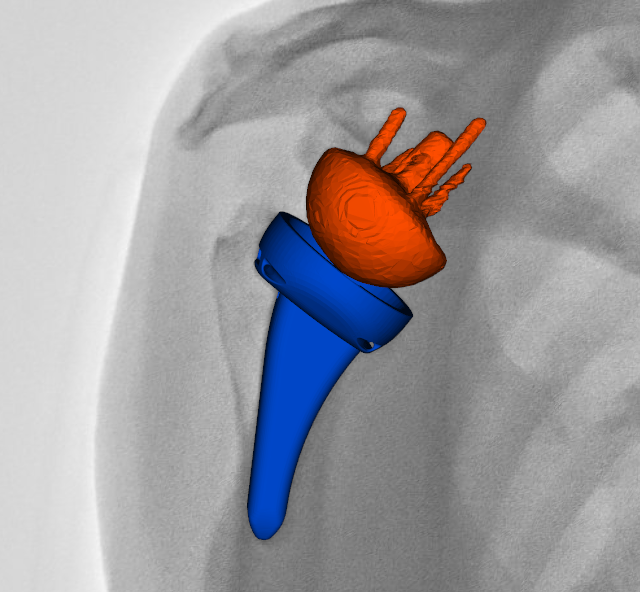
\includegraphics[width=0.3\textwidth]{~/figures/raster/TSA_original.png}
	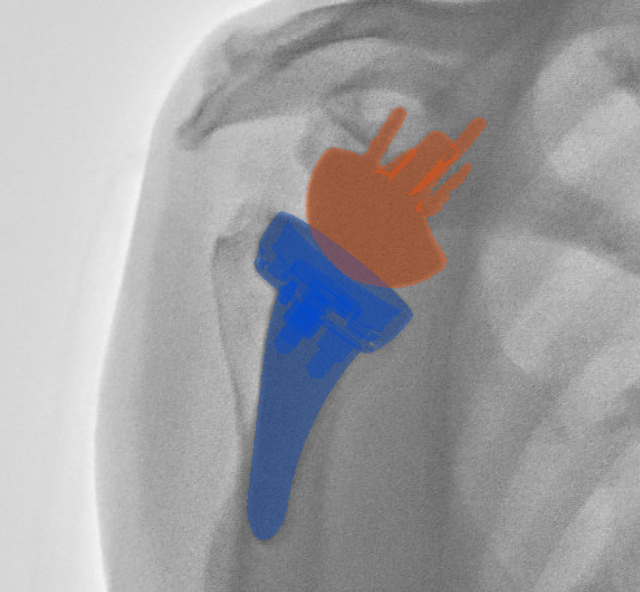
\includegraphics[width=0.3\textwidth]{~/figures/raster/TSA_transparent.png}
	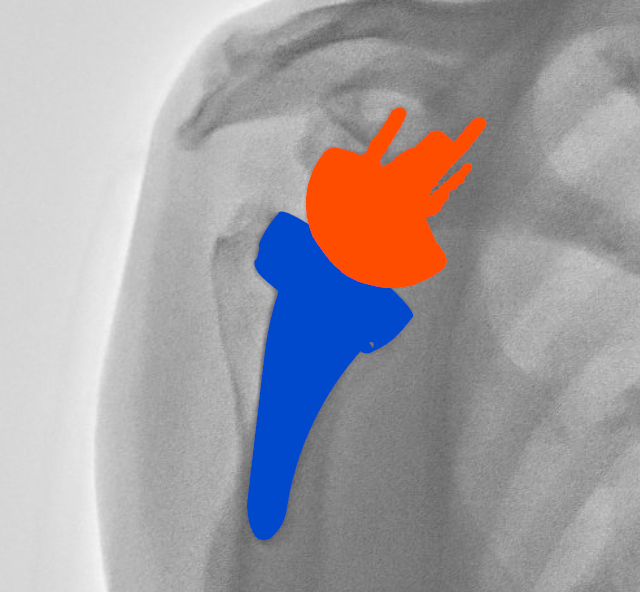
\includegraphics[width=0.3\textwidth]{~/figures/raster/TSA_solid.png}
	\caption{Some different model views of a manually registered humeral and glenoid implant in an rTSA system. Of note, each view gives the user a different type of feature to focus on. The original view allows the user to determine the relative orientation based on shading, the transparent view allows the user to see the underlying fluoroscopic image, and the solid view allows the user to focus on specific regions of error. Each is crucial to performing manual registration.}
	\label{fig:TSA-multiview}
\end{figure}

The current investigation delves into the fundamental shape aspects of each arthroplasty system, with a focus on developing a method for autonomously measuring rTSA kinematics from single-plane fluoroscopy.
Central to this is the use of Invariant Shape Descriptors, particularly the Invariant Angular Radial Transform Descriptor (IARTD), which offers a mathematically robust approach to describe object shapes \cite{leeNewShapeDescription2012}.
These descriptors are immune to variations in scale, translation, or orientation \cite{zhangReviewShapeRepresentation2004}, and are adept at quantifying the relative ``nearness'', ``farness'', and ``uniqueness'' of shapes as vector differences.
Such properties are valuable for object categorization \cite{richardIdentificationThreeDimensionalObjects1974,wallaceAnalysisThreedimensionalMovement1980,wallaceEfficientThreedimensionalAircraft1980} and kinematics measurement \cite{banksAccurateMeasurementThreedimensional1996}, with IARTD's sensitivity to radial shape differences \cite{leeNewShapeDescription2012} being particularly beneficial for detailed contour analysis.

The focus of this analysis is on the sensitivity of projected 2D shapes, as depicted by IARTD, to changes in their 3D orientation.
This is key to understanding the impact of subtle orientation variations on the projected shape, an aspect integral to shape-based optimization metrics.
The ultimate aim is to highlight performance differences in autonomous kinematics measurements between TKA and rTSA implant systems.
Additionally, the study seeks to identify areas where imaging methods can be improved to boost the algorithm's performance.

%%% Local Variables:
%%% mode: latex
%%% TeX-master: "../Jensen_Shape_Sensitivity"
%%% End:
